

% SINDA 
\begin{frame}[ctb!]
  \frametitle{Background: Numerical SINDA{\textbackslash}G Model}
  A model created by the UFD team at Argonne national lab using the 
  SINDA{\textbackslash}G heat transport framework employs a lumped parameter 
  model and an optimization loop to arrive at a minimal drift spacing for a 
  given waste stream in agreement with user input thermal limits. 
  \begin{figure}[h!]
    \begin{center}
      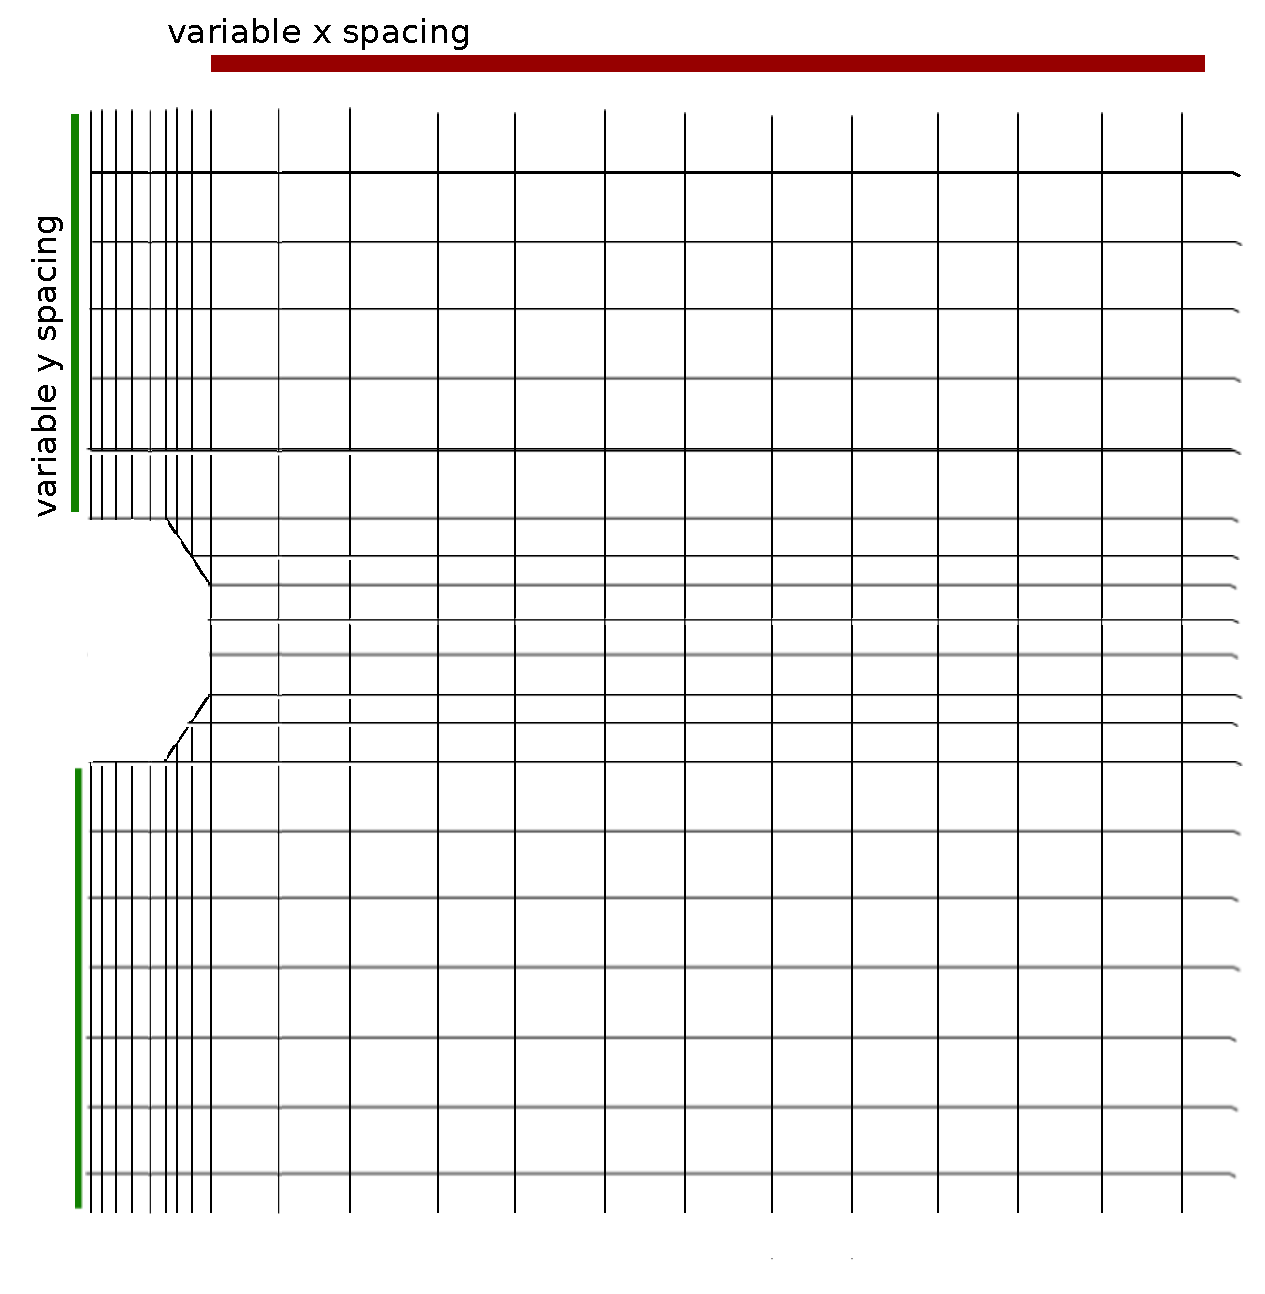
\includegraphics[height=.5\textheight]{sindageom.eps}
    \end{center}
    \caption{Two adjustable geometric dimensions of the ANL model.} 
    \label{fig:sindageom}
  \end{figure}
\end{frame}


\begin{frame}[ctb!]
  \frametitle{Numerical Model : Lumped Parameter Technique}
  % resistor diagram
  \begin{figure}[h!]
    \begin{center}
      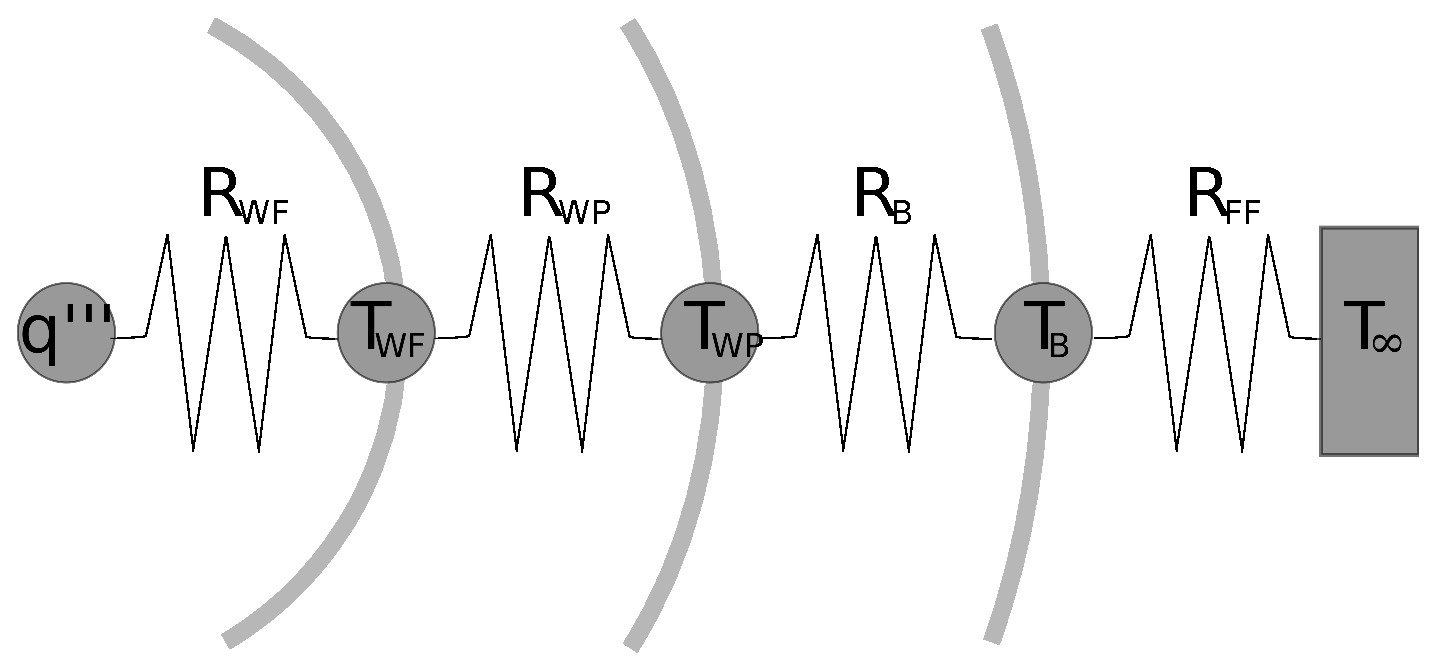
\includegraphics[width=0.9\textwidth]{lumpedParam.eps}
    \end{center}
    \caption{The lumped parameter analogy used for heat transfer can be applied 
    as a one dimensional approximation to the disposal system concept. }
    \label{fig:lumpedParam}
  \end{figure}
\end{frame}

%%%%%%%%%%%%%%%%%%%%%%%%%%%%%%%%%%%%%%%%%%%%%%%%%%%%%%%%%%%%%%%%%%%%%%%%%%%%%%%%

%% The ANL model

\begin{frame}[ctb!]
\frametitle{Calculation Method}

The SINDA{\textbackslash}G  calculation engine uses a lumped parameter numeric model.
Originally created for optimal waste loading analysis of the Yucca Mountain 
Repository, the 
model for an array of drifts is geometrically adjustable,  as illustrated in 
Figure \ref{fig:sindageom}. 

\begin{figure}[htbp!]
  \begin{center}
    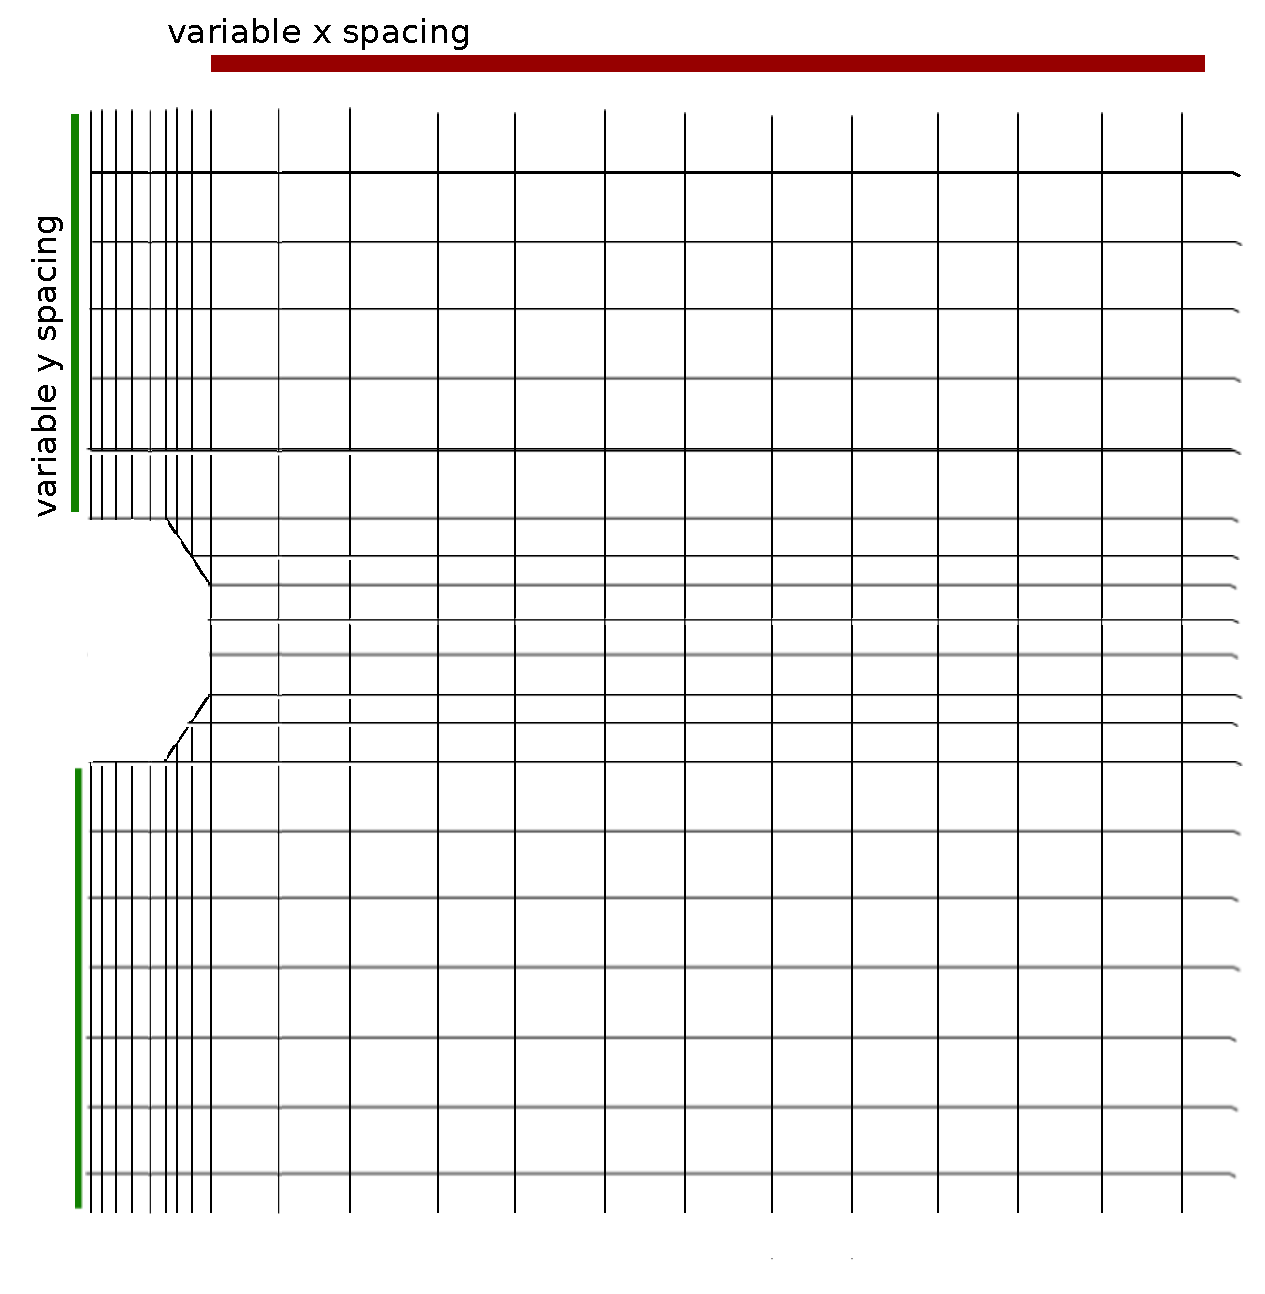
\includegraphics[width=0.4\textwidth]{./sindageom.eps}
  \end{center}
  \caption{The geometry of the 2D thermal model can be adjusted by altering 
  tunnel diameter, tunnel spacing, and the vertical distance below the surface.}
  \label{fig:sindageom}
\end{figure}
\end{frame}

\begin{frame}[ctb!]
\frametitle{Calculation Method}
The SINDA{\textbackslash}G  lumped capacitance tool solves a thermal circuit, for which 
conducting nodes may be of four types corresponding to the four modes of heat 
transfer. Nodes are connected by conduction, convection, radiation, and mass 
flow heat transfer links. In the SINDA{\textbackslash}G engine, these are represented by
\footnotesize{
\begin{align}
  R_{rad}  &= \frac{1}{\sigma F_{ij}A\left[ T_i + T_A + T_j + T_A 
  \right]\left[(T_i+T_A)^2+(T_j+T_A)^2\right]}\nonumber\\
  R_{cond} &= \frac{L}{K_{th} A}\mbox{, }R_{conv} = \frac{1}{h A}\mbox{, and 
  }R_{mf} = \frac{1}{\dot{m}c_p}
  \intertext{where}
  K_{th}&= ~~\mbox{thermal conductivity}[W\cdot m^{-1}\cdot K^{-1}]\nonumber\\
  A&= ~~\mbox{area} [m^2]\nonumber\\
  c_p&=~~\mbox{specific heat capacity} [J\cdot K^{-1}]\nonumber  \\
  h&= ~~\mbox{heat transfer coefficient}[W\cdot m^{-1} \cdot K^{-1}]\nonumber \\
  \dot{m}&= ~~\mbox{mass transfer rate}[kg\cdot s^{-1}]\nonumber \\
  T_i&= ~~\mbox{lump temperature} [^{\circ}C] \nonumber\\
  T_A&= ~~\mbox{absolute temperature} [^{\circ}C] \nonumber\\
  F_{ij}&= ~~\mbox{radiation interchange factor} [-] .\nonumber
\end{align}
}
\end{frame}


\begin{frame}[ctb!]
  \frametitle{SINDA{\textbackslash}G Geometries}

Two SINDA{\textbackslash}G model geometries have been used in this benchmark.  
\begin{itemize}
  \item{Single Drift} In the single drift geometry, there is a distant fixed boundary condition and one waste tunnel is modeled with a continuous, cylindrical heat source of infinite length. The linear heat source in $[\frac{W}{m}]$ is modeled as if it is spread azimuthally over the surface of the drift tunnel.  
  \item{Multiple Drift} As llustrated in Figure \ref{fig:sindageom}, an infinite array of identical single-drift heat sources is modeled, by assuming one-half of a storage tunnel with a reflective boundary condition at a vertical plane midway between drifts. 
\end{itemize}

\end{frame}
